% Paper for CGAT
\documentclass[10pt, conference, compsocconf]{IEEEtran}

\usepackage{float}
%\usepackage{url}
\usepackage{graphicx}
\usepackage{subfig}
\usepackage{color}

\begin{document}

\title{CGAT In The Hat}

% author names and affiliations
% use a multiple column layout for up to two different
% affiliations

\author{\IEEEauthorblockN{Eriq Augustine, Ryan Hnarkis, Aldrin Montana, Ryan Verdon, Tyler Yero}
\\
\IEEEauthorblockA{Department of Computer Science\\
Cal Poly, San Luis Obispo\\
 \textsf{\{eaugusti, rhnaraki, amontana, rverdon, tyero\}@calpoly.edu}
}
}

\maketitle

\thispagestyle{empty}
\pagestyle{empty}

\section{Introduction}\label{sec:introduction}
Gene annotation is the process of associating metadata about a gene with the
contig, a dna sequence, on which the gene resides. This metadata is necessary for conducting
genomic research projects and analysis involving the contig's genomic sequence.
Currently, there is no specialty gene annotation software. Genome browsers
all maintain lots of genomic data and are used when manually annotating genes,
but do not provide a user-friendly interface. While genome browsers
will likely never be replaced (UCSC genome browser, etc. are well
established), it would be desirable to have a software system that better
accommodates the visual and informational needs of gene annotation.

\textit{CGAT} is a web-based gene annotation application designed with
usability, simplicity, and efficiency in mind. It is not a feature and data
rich genome browser like the \textit{UCSC genome brower}. Nor is \textit{CGAT}
designed to be a replacement for other genome browsers in any aspect other than
gene annotation. Other gene browsers attempt to accommodate many needs of the
biology community and so offer many features, and a cluttered, chaotic
interface. Gene annotation, while not a trivial task, can be well-serviced by a
simple data model. Ideally, by focusing on a simple data model, \textit{CGAT}
is able to provide a clean, streamlined experience. \textit{CGAT} aims to
provide users with a way to view gene annotations without extra, unnecessary
information obscuring their view while also embodying a Wikipedia-like emphasis
on collaboration and openness.

%Anya Goodman, a professor in the biochemistry department at Cal Poly, San Luis
%Obispo, offers a bioinformatics course that covers several aspects of gene
%annotation. This project is spearheaded by Ryan Verdon to accommodate Dr.
%Goodman's needs and ideas for ideal gene annotation software.

This paper primarily focuses on considerations for \textit{CGAT}s database
architecture. These considerations are made with regards to a MySQL cluster
versus a Couchbase cluster to determine which database architecture is most
efficient for running \textit{CGAT}. Section \ref{sec:motive} discusses our
motivation to compare Couchbase and MySQL in this paper, while section
\ref{sec:design} talks about how we designed experimental workloads to use for
our comparison of Couchbase vs MySQL. In section \ref{sec:workload} we
describe the workloads and how they are relevant to \textit{CGAT}, some brief
implementation details are outlined in section \ref{sec:implementation}, we
evaluate our results in section \ref{sec:eval} and finally conclude in
section \ref{sec:conclusions}.

\section{Motivation}\label{sec:motive}
Traditional web applications are almost always backed by a relational database.
However, there has been a recent movement towards the use of NoSQL databases for
web applications. Our main goal is to determine whether a NoSQL database, Couchbase,
can outperform a traditional relational database, MySQL, for \textit{CGAT}'s
common operations.

\onecolumn
\appendices

\section{JSON Data Models}\label{sec:data_models}
\centering
Here are diagrams depicting our JSON data model.

\begin{figure*}[t]
   \centering
   \subfloat[Contig format]{\label{fig:JSON-contig}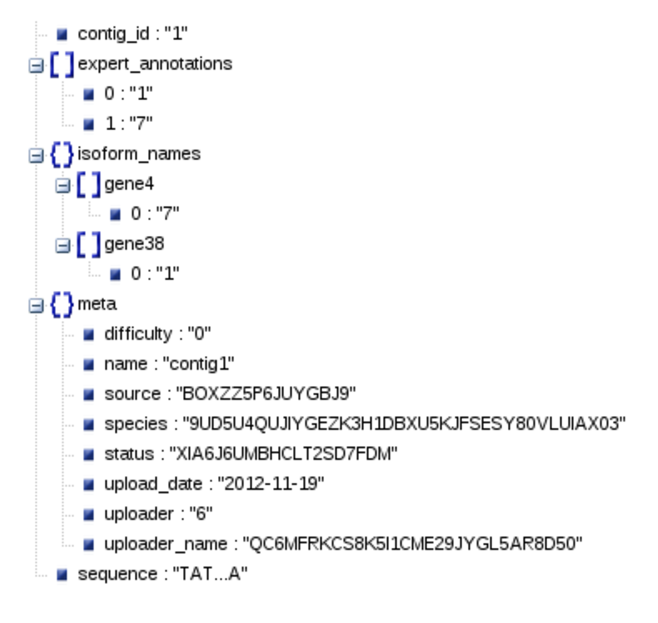
\includegraphics[height=70mm]{contig.eps}}
   \subfloat[Annotation format]{\label{fig:JSON-annotation}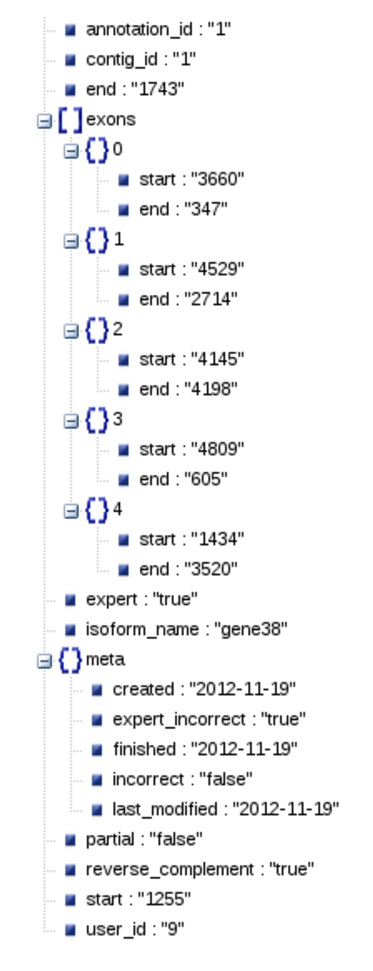
\includegraphics[height=80mm]{annotation.eps}}
   \caption{JSON format for Contigs and Annotations.}
\end{figure*}

\begin{figure*}[t]
   \centering
   \subfloat[User format]{\label{fig:JSON-user}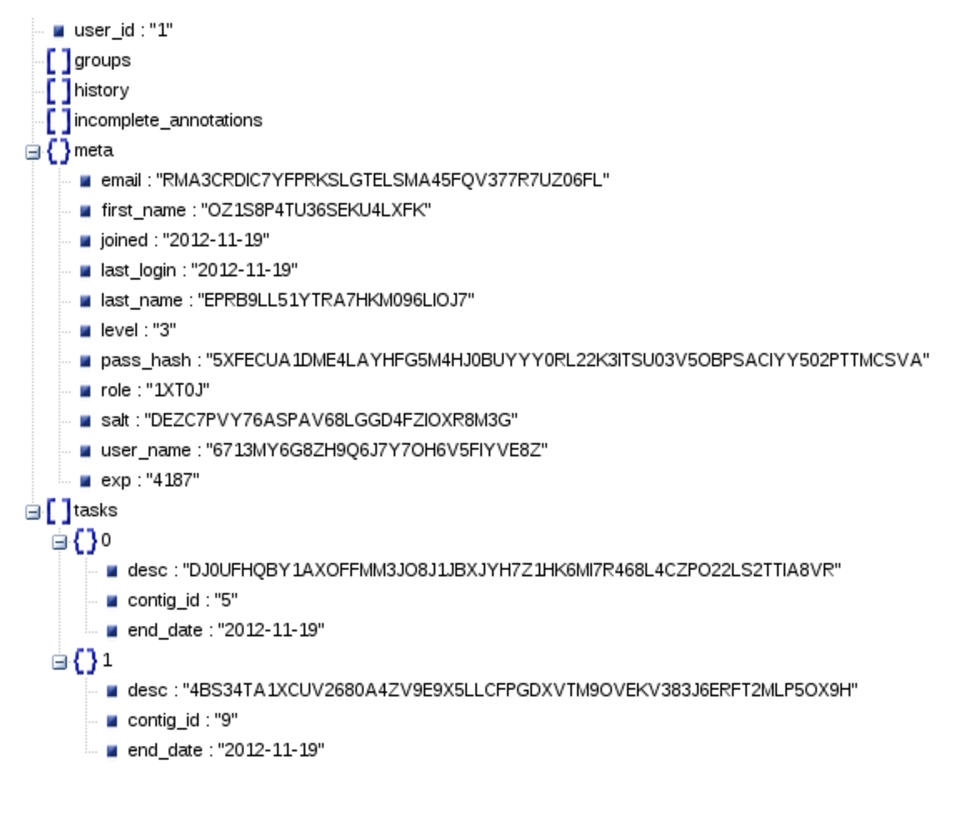
\includegraphics[height=90mm]{user.eps}}
   \subfloat[Group format]{\label{fig:JSON-group}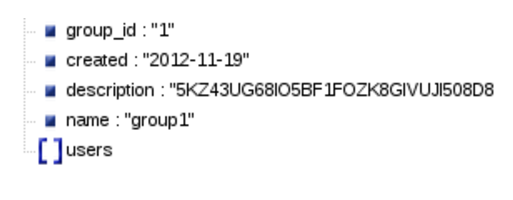
\includegraphics[height=25mm]{group.eps}}
   \caption{JSON format for Users and Groups.}
\end{figure*}

%\begin{figure*}
%  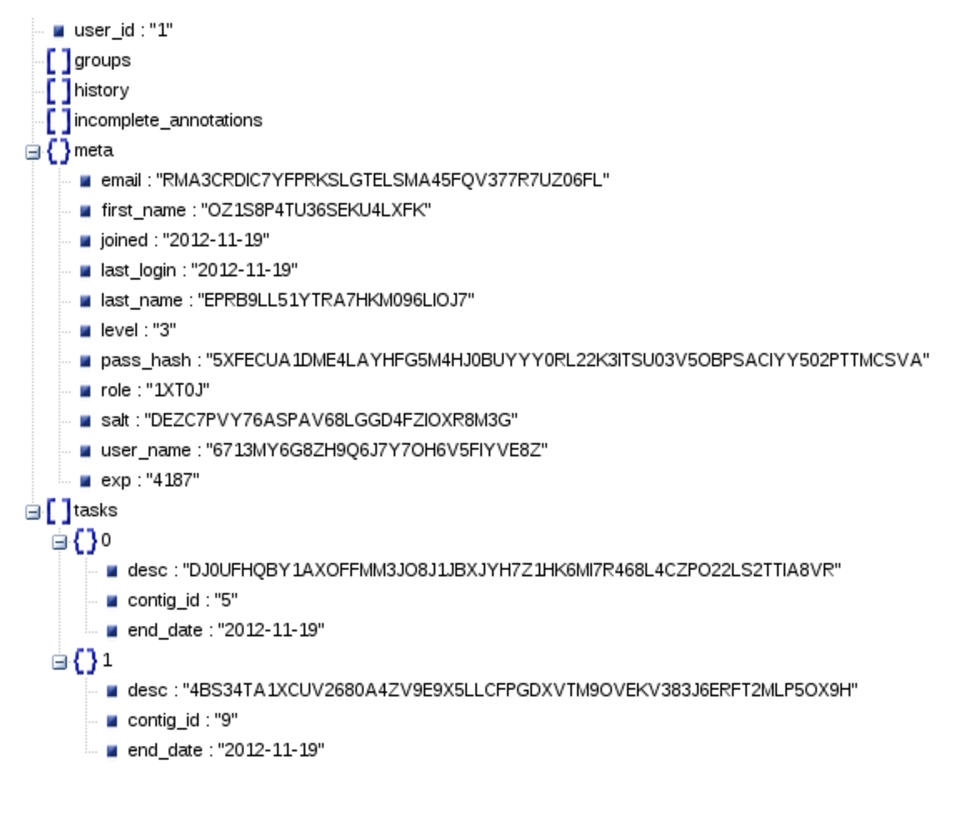
\includegraphics[height=90mm]{user.eps}
%	\caption{The JSON for a user.}
%	\label{fig:JSON-user}
%\end{figure*}
%\begin{figure*}
%  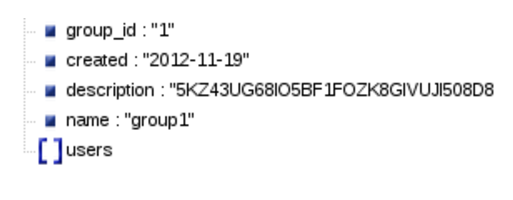
\includegraphics[height=25mm]{group.eps}
%	\caption{The JSON for a group.}
%	\label{fig:JSON-group}
%\end{figure*}
%\begin{figure*}
%  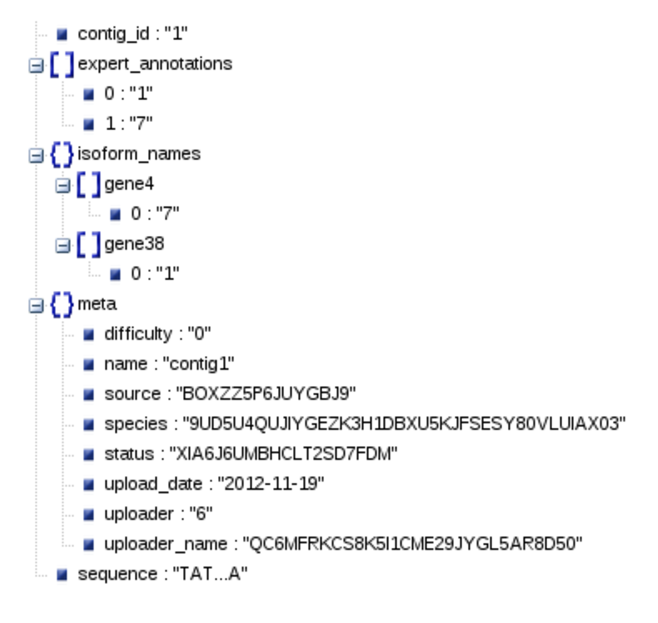
\includegraphics[height=80mm]{contig.eps}
%  \caption{The JSON for a contig.}
%  \label{fig:JSON-contig}
%\end{figure*}
%\begin{figure*}
%  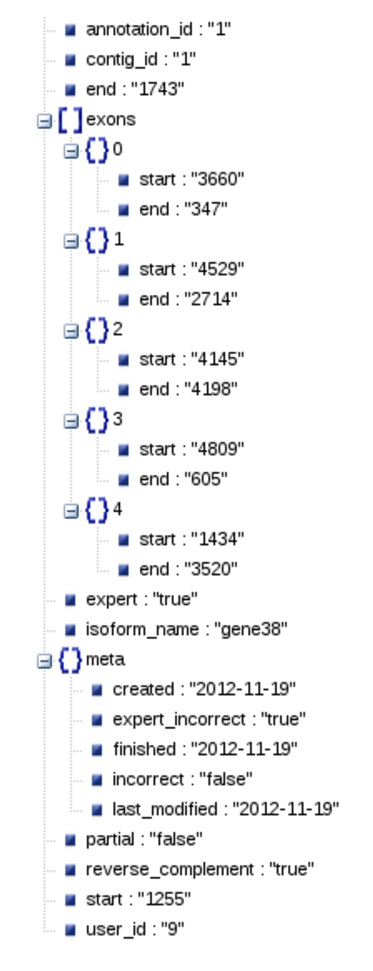
\includegraphics[height=90mm]{annotation.eps}
%	\caption{The JSON for an annotation.}
%	\label{fig:JSON-annotation}
%\end{figure*}

% TODO: Uncomment if we use any refs
% \bibliographystyle{acm}
% \bibliography{refs}

\end{document}
